\makeatletter
\def\input@path{{../}}
\makeatother

\documentclass[/main.tex]{subfiles}
\graphicspath{{./pics/}{appAllResults/pics/}}
\begin{document}

\newcommand{\allmodeplots}[3]{% inputs are file name modifier, description of mode, and discription of gamma

  \begin{sidewaystable}[p]
    \caption[#3 of #2: Energy systematics table]{ \label{tab:energysystematics}
      Table of energy estimation uncertainties for the #3 from the #2 decay mode
    }
    \resizebox{\textwidth}{!}{%
      \input{appAllResults/tables/table_#1_pseff.tex} }
  \end{sidewaystable}
  
  \begin{figure}[!htb]
    \centering
    \subfloat[Simulated BG Sum Energy Spectrum]{\includegraphics[width=.5\linewidth]{BGSumECuts_#1}}
    \subfloat[Simulated ES Sum Energy Spectrum]{\includegraphics[width=.5\linewidth]{ESSumECuts_#1}}\\
    \subfloat[Simulated BG Coincident Energy Spectrum]{\includegraphics[width=.5\linewidth]{BGCoinECuts_#1}}
    \subfloat[Simulated ES Coincident Energy Spectrum]{\includegraphics[width=.5\linewidth]{ESCoinECuts_#1}}
    \caption[#3 of #2: Sum and coincident simulated energy spectra with cuts]{
      Sum energy and coincident energy spectra for events in the ROIs
    }
  \end{figure}
  
  \begin{figure}[!htb]
    \centering
    \includegraphics[width=0.8\linewidth]{BG2Dcuts_#1}
    \caption[#3 of #2: 2D plot of simulated sum and coincident energy cuts]{
      Simulated multiplicity 2 energy spectrum with sum and coincident energy cuts included.
    }
  \end{figure}

  \begin{figure}[!htb]
    \centering
    \includegraphics[width=0.8\linewidth]{ESAllCuts_#1}
    \caption[#3 of #2: Effect of all cuts in ROI]{Effect of all cuts in ROI}
  \end{figure}

  \begin{table}[!htb]
    \centering
    \input{appAllResults/tables/table_#1_efficiency.tex}
    \caption[#3 of #2: Table of efficiencies]{\label{tab:eff_#1}
      Table of detection efficiencies
    }
  \end{table}

  \begin{figure}[!htb]
    \centering
    \includegraphics[width=0.8\linewidth]{Data2Dcuts_#1}
    \caption[#3 of #2: 2D plot of cuts applied to data]{
      All measured multiplicity 2 events with sum and coincident energy cuts included
    }
  \end{figure}

  \begin{figure}[!htb]
    \centering
    \subfloat[Simulated BG Cuts]{\includegraphics[width=.5\linewidth]{BGAllCuts_#1}}
    \subfloat[Data Cuts]{\includegraphics[width=.5\linewidth]{DataAllCuts_#1}}
    \caption[#3 of #2: Cuts appliled to simulated and measured background data]{
      Effect of all cuts applied to measured and simulated background data.
    }
  \end{figure}
  
  \begin{sidewaystable}[p]
    \centering
    \input{appAllResults/tables/table_#1_bgcuts.tex}
    \caption[#3 of #2: Summary of cut efficiency in BG and data]{
      Table of cut descriptions and efficiencies for simulated backgrounds and measured data.
    }
  \end{sidewaystable}
  
  \begin{figure}[!htb]
    \centering
    \includegraphics[width=0.8\linewidth]{DataROIs_#1}
    \caption[#3 of #2: Background spectrum after all cuts with ROIs drawn on]{
      Background spectrum after all cuts have been applied, with ES and ROI backgrounds.
    }
  \end{figure}
}

\onlyinsubfile{\appendix}
\chapter{Detailed Results for All Decay Modes}
\label{app:allresults}

The main document concerned itself primarily with the \tnbb\ of \Ge{76} to the \SP{0}{+}{1} excited state.
However, results are presented for all decay modes and energy peaks.
This appendix will present figures and tables detailing the simulations, cuts, efficiencies and results for each decay mode and peak.

\section{\tnbb\ to \SP{0}{+}{1}}
Note that both the 559~and 563~keV peaks will be shown together since they use the same sets of cuts.
\begin{figure}[!htb]
  \centering
  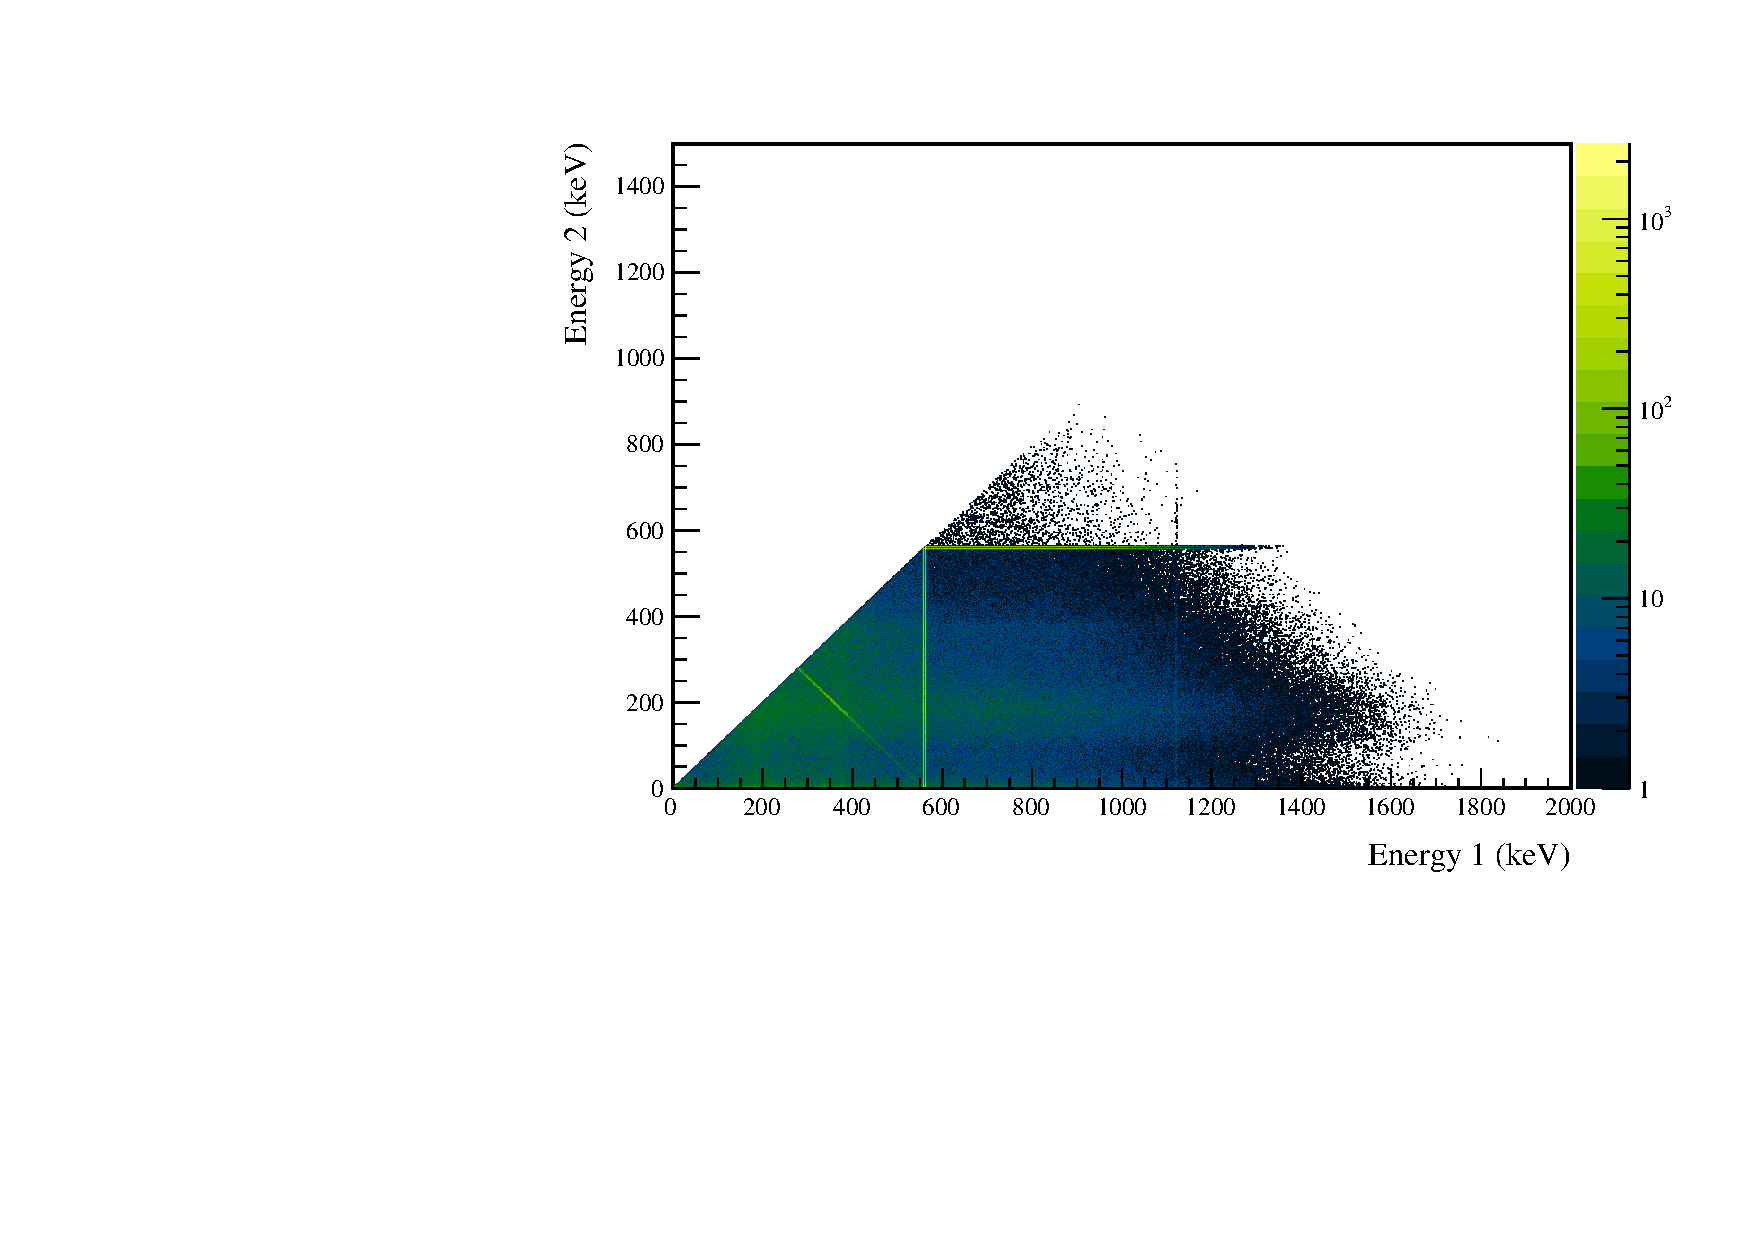
\includegraphics[width=.8\linewidth]{ESsim_2vBB_ES0_1}
  \caption[Simulation of \tnbb\ to \SP{0}{+}{1}]{
    Simulated multiplicity 2 energy spectrum of the \tnbb\ to \SP{0}{+}{1} decay mode}
\end{figure}

\allmodeplots{2vBB_ES0_1}{\tnbb\ to \SP{0}{+}{1}}{559~and 563~keV $\gamma$s}

\section{\tnbb\ to \SP{2}{+}{1}}
\begin{figure}[!htb]
  \centering
  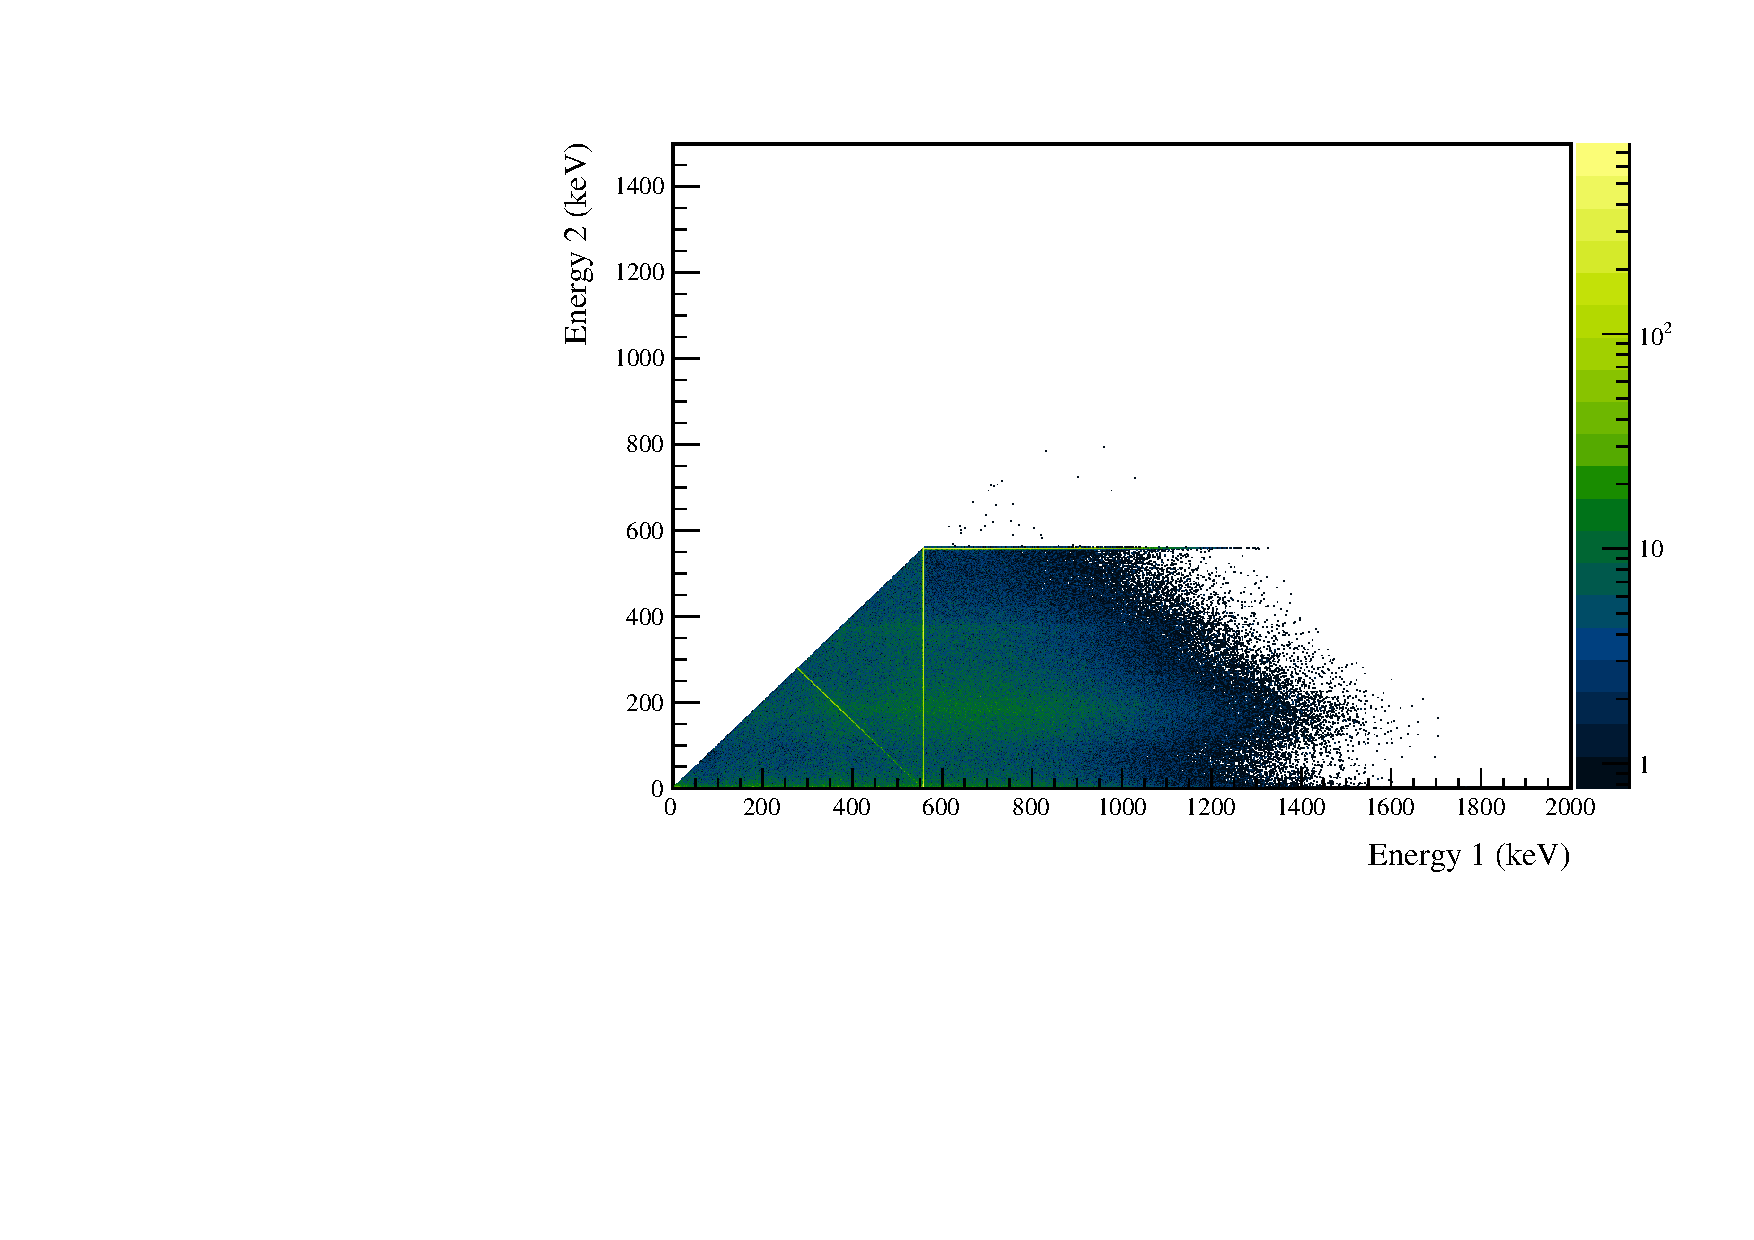
\includegraphics[width=.8\linewidth]{ESsim_2vBB_ES2_1}
  \caption[Simulation of \tnbb\ to \SP{2}{+}{1}]{
    Simulated multiplicity 2 energy spectrum of the \tnbb\ to \SP{2}{+}{1} decay mode}
\end{figure}

\allmodeplots{2vBB_ES2_1}{\tnbb\ to \SP{2}{+}{1}}{559~keV $\gamma$}

\section{\tnbb\ to \SP{2}{+}{2}}
\begin{figure}[!htb]
  \centering
  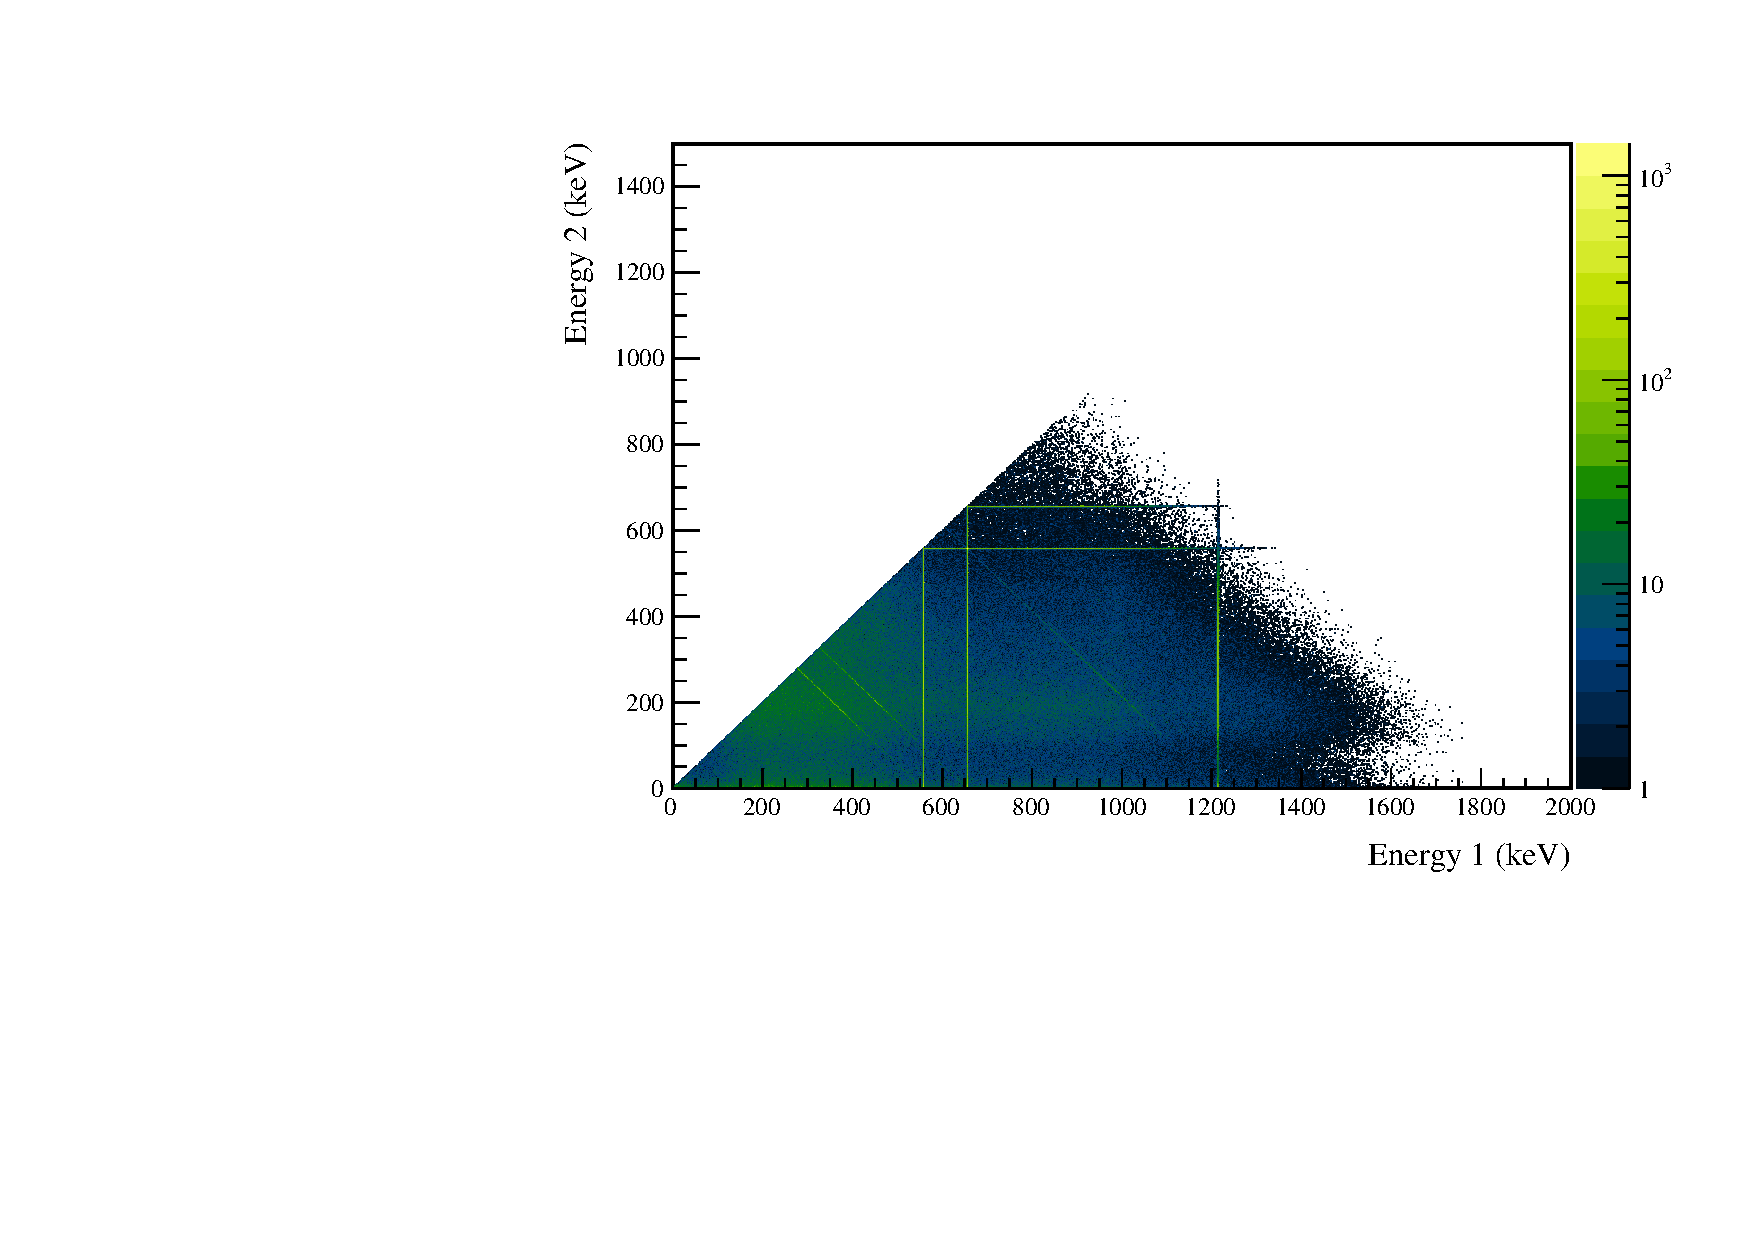
\includegraphics[width=.8\linewidth]{ESsim_2vBB_ES2_2}
  \caption[Simulation of \tnbb\ to \SP{2}{+}{2}]{
    Simulated multiplicity 2 energy spectrum of the \tnbb\ to \SP{2}{+}{2} decay mode}
\end{figure}

\subsection{559 keV peak}
\allmodeplots{2vBB_ES2_2_559}{\tnbb\ to \SP{2}{+}{2}}{559~keV $\gamma$}
\subsection{657 keV peak}
\allmodeplots{2vBB_ES2_2_657}{\tnbb\ to \SP{2}{+}{2}}{657~keV $\gamma$}
\subsection{1216 keV peak}
\allmodeplots{2vBB_ES2_2_1216}{\tnbb\ to \SP{2}{+}{2}}{1216~keV $\gamma$}


\end{document}